\section{Slice Layouts}
    \subsection{PIN Slice Layout}
        \begin{figure}[H]
            \centering
            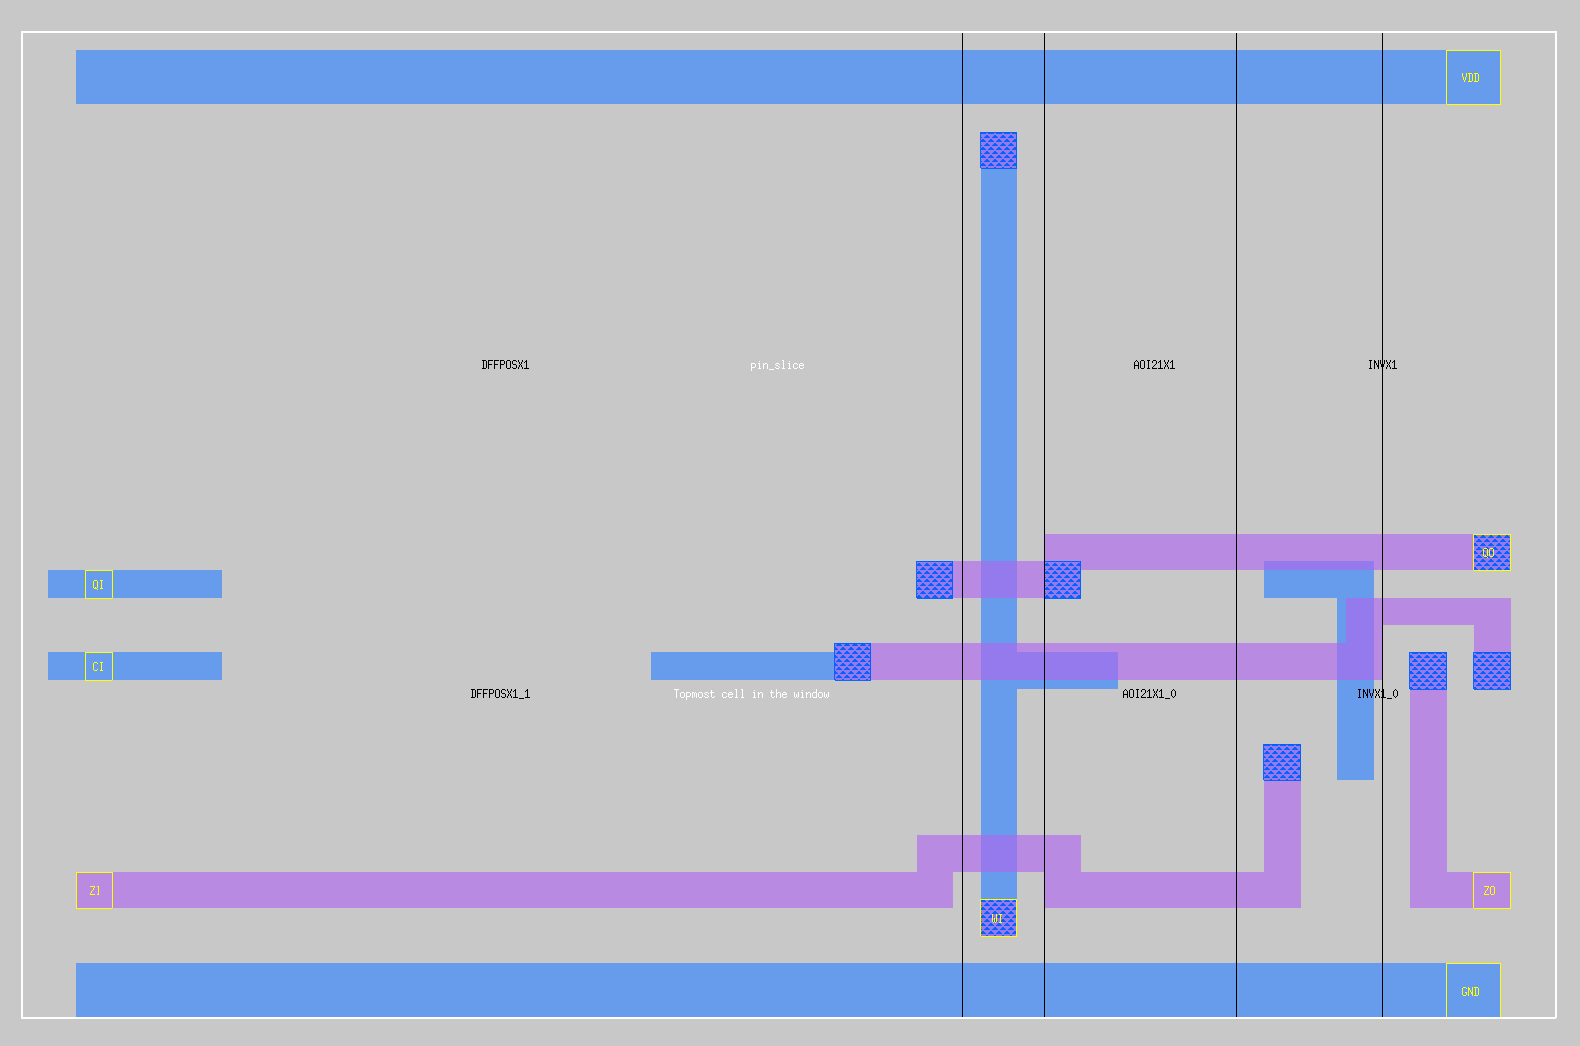
\includegraphics[width=0.75\linewidth]{../../magic/images/pin_slice.png}
            \caption{PIN Slice Layout}
        \end{figure}
        \begin{figure}[H]
            \centering
            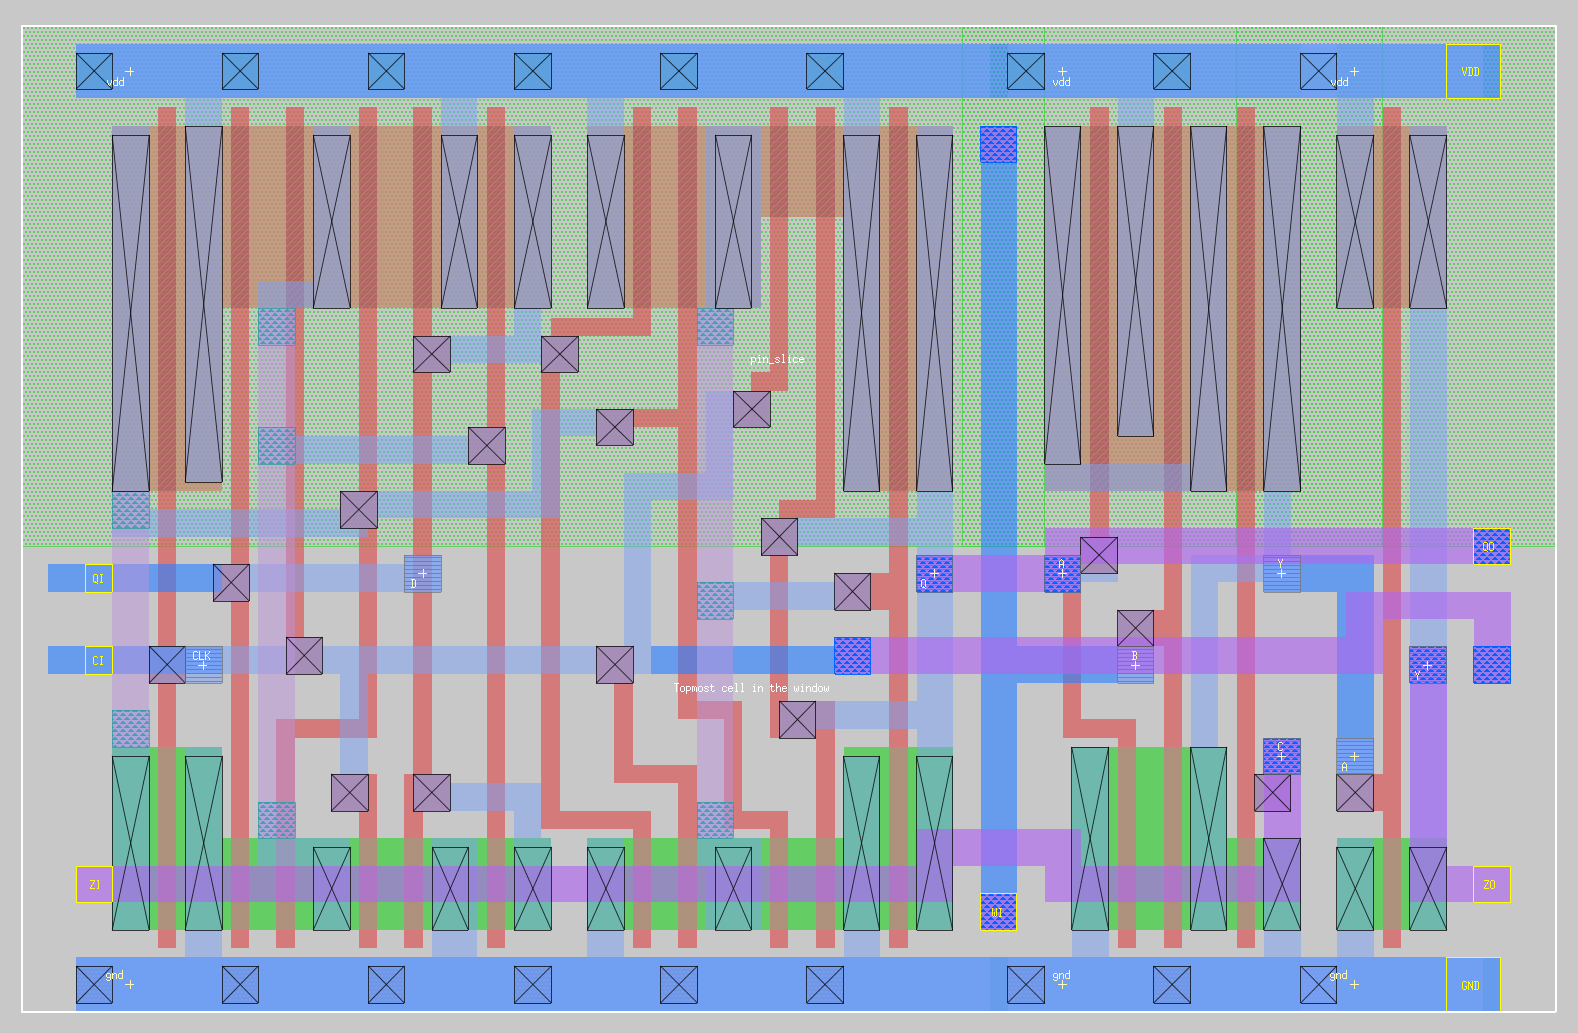
\includegraphics[width=0.75\linewidth]{../../magic/images/pin_slice_internal.png}
            \caption{PIN Slice Layout Internal}
        \end{figure}
    \subsection{Shift Slice Layout}
        \begin{figure}[H]
            \centering
            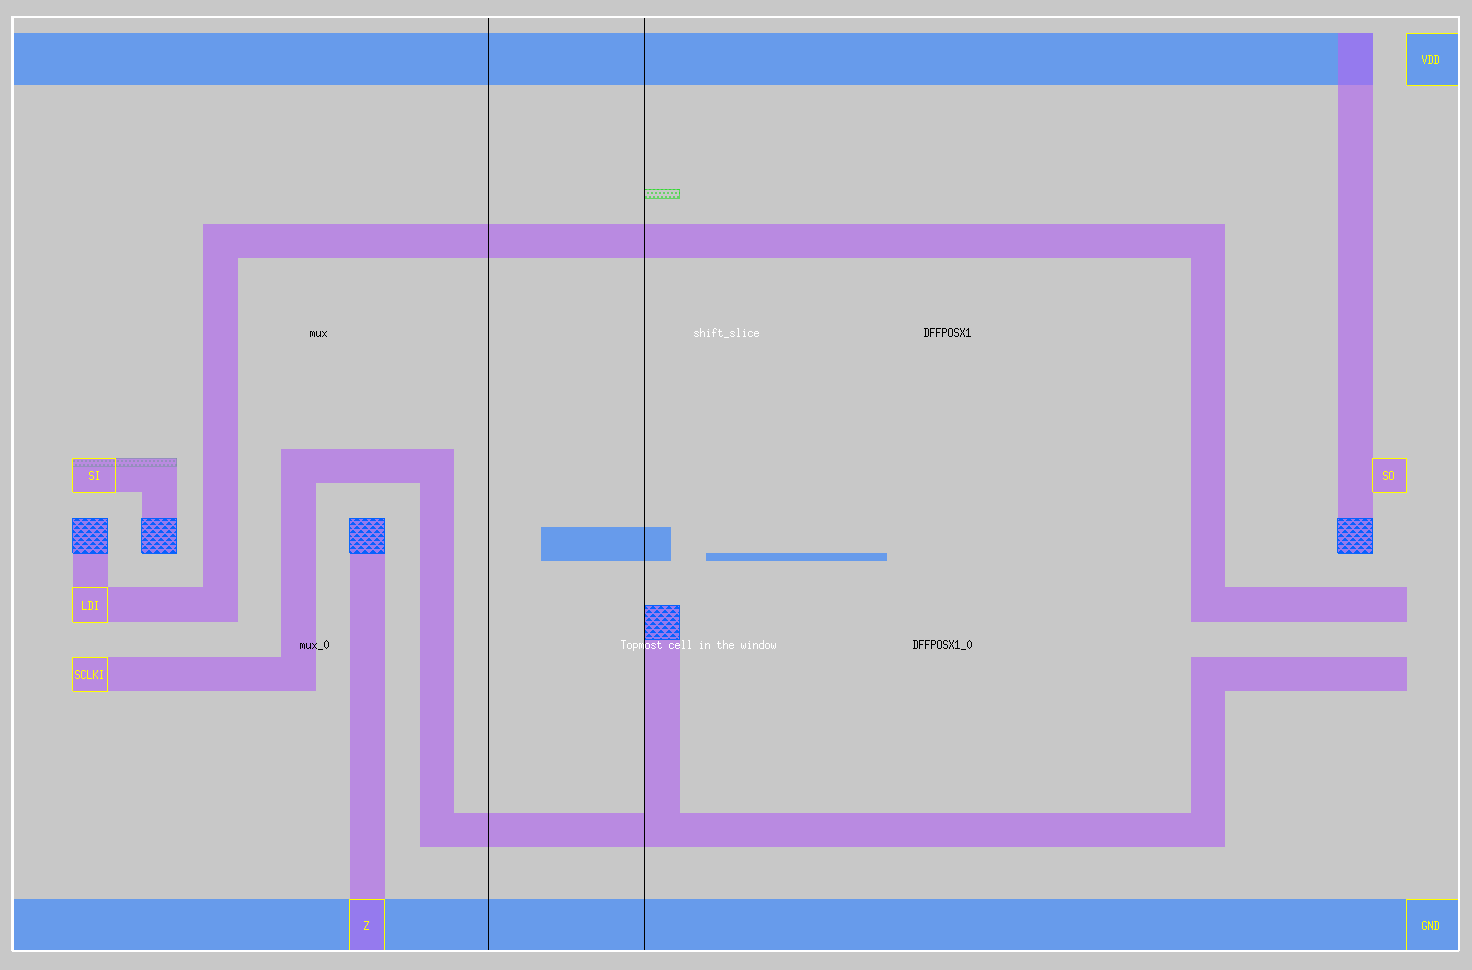
\includegraphics[width=0.75\linewidth]{../../magic/images/shift_slice.png}
            \caption{PIN Slice Layout}
        \end{figure}
        \begin{figure}[H]
            \centering
            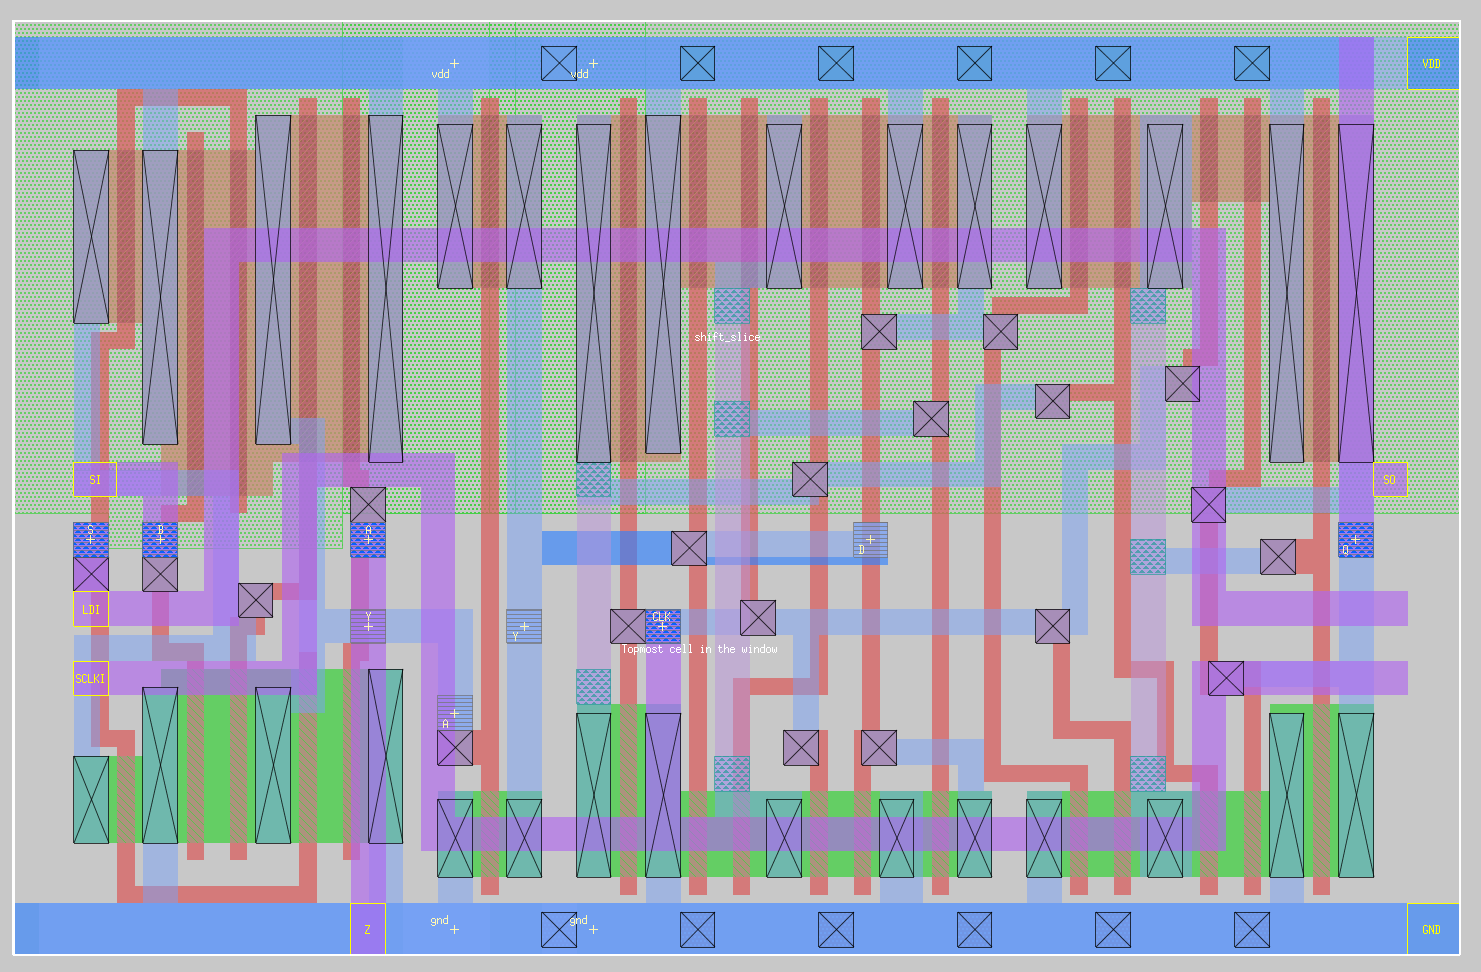
\includegraphics[width=0.75\linewidth]{../../magic/images/shift_slice_internal.png}
            \caption{PIN Slice Layout Internal}
        \end{figure}

\newpage
\section{Slice IRSIM Results}
    \subsection{PIN Slice IRSIM Results}
        \lstinputlisting[caption=Python PIN Slice IRSIM CMD File Generator, language=Python]{../../irsim/pin_slice.py}
        \begin{figure}[H]
            \centering
            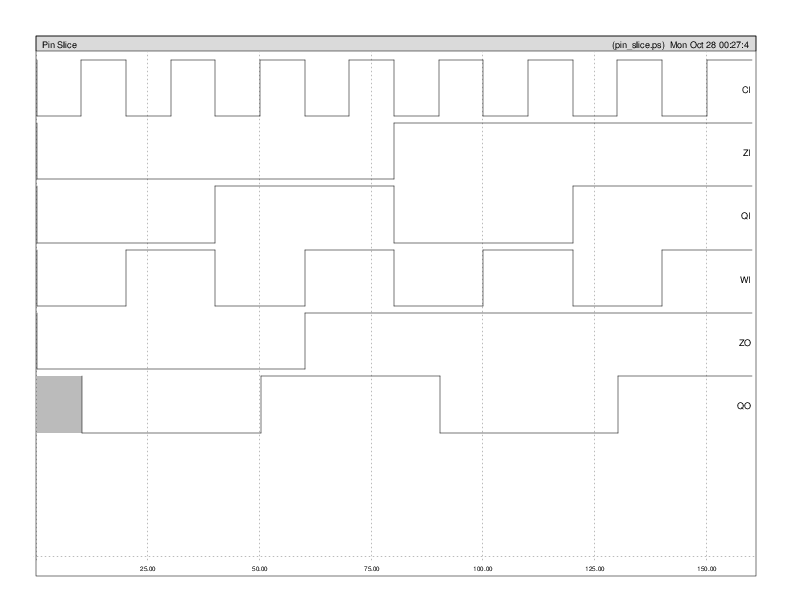
\includegraphics[width=0.75\linewidth]{../../irsim/pin_slice.png}
            \caption{PIN Slice IRSIM Functional Results}
        \end{figure}
        \begin{figure}[H]
            \centering
            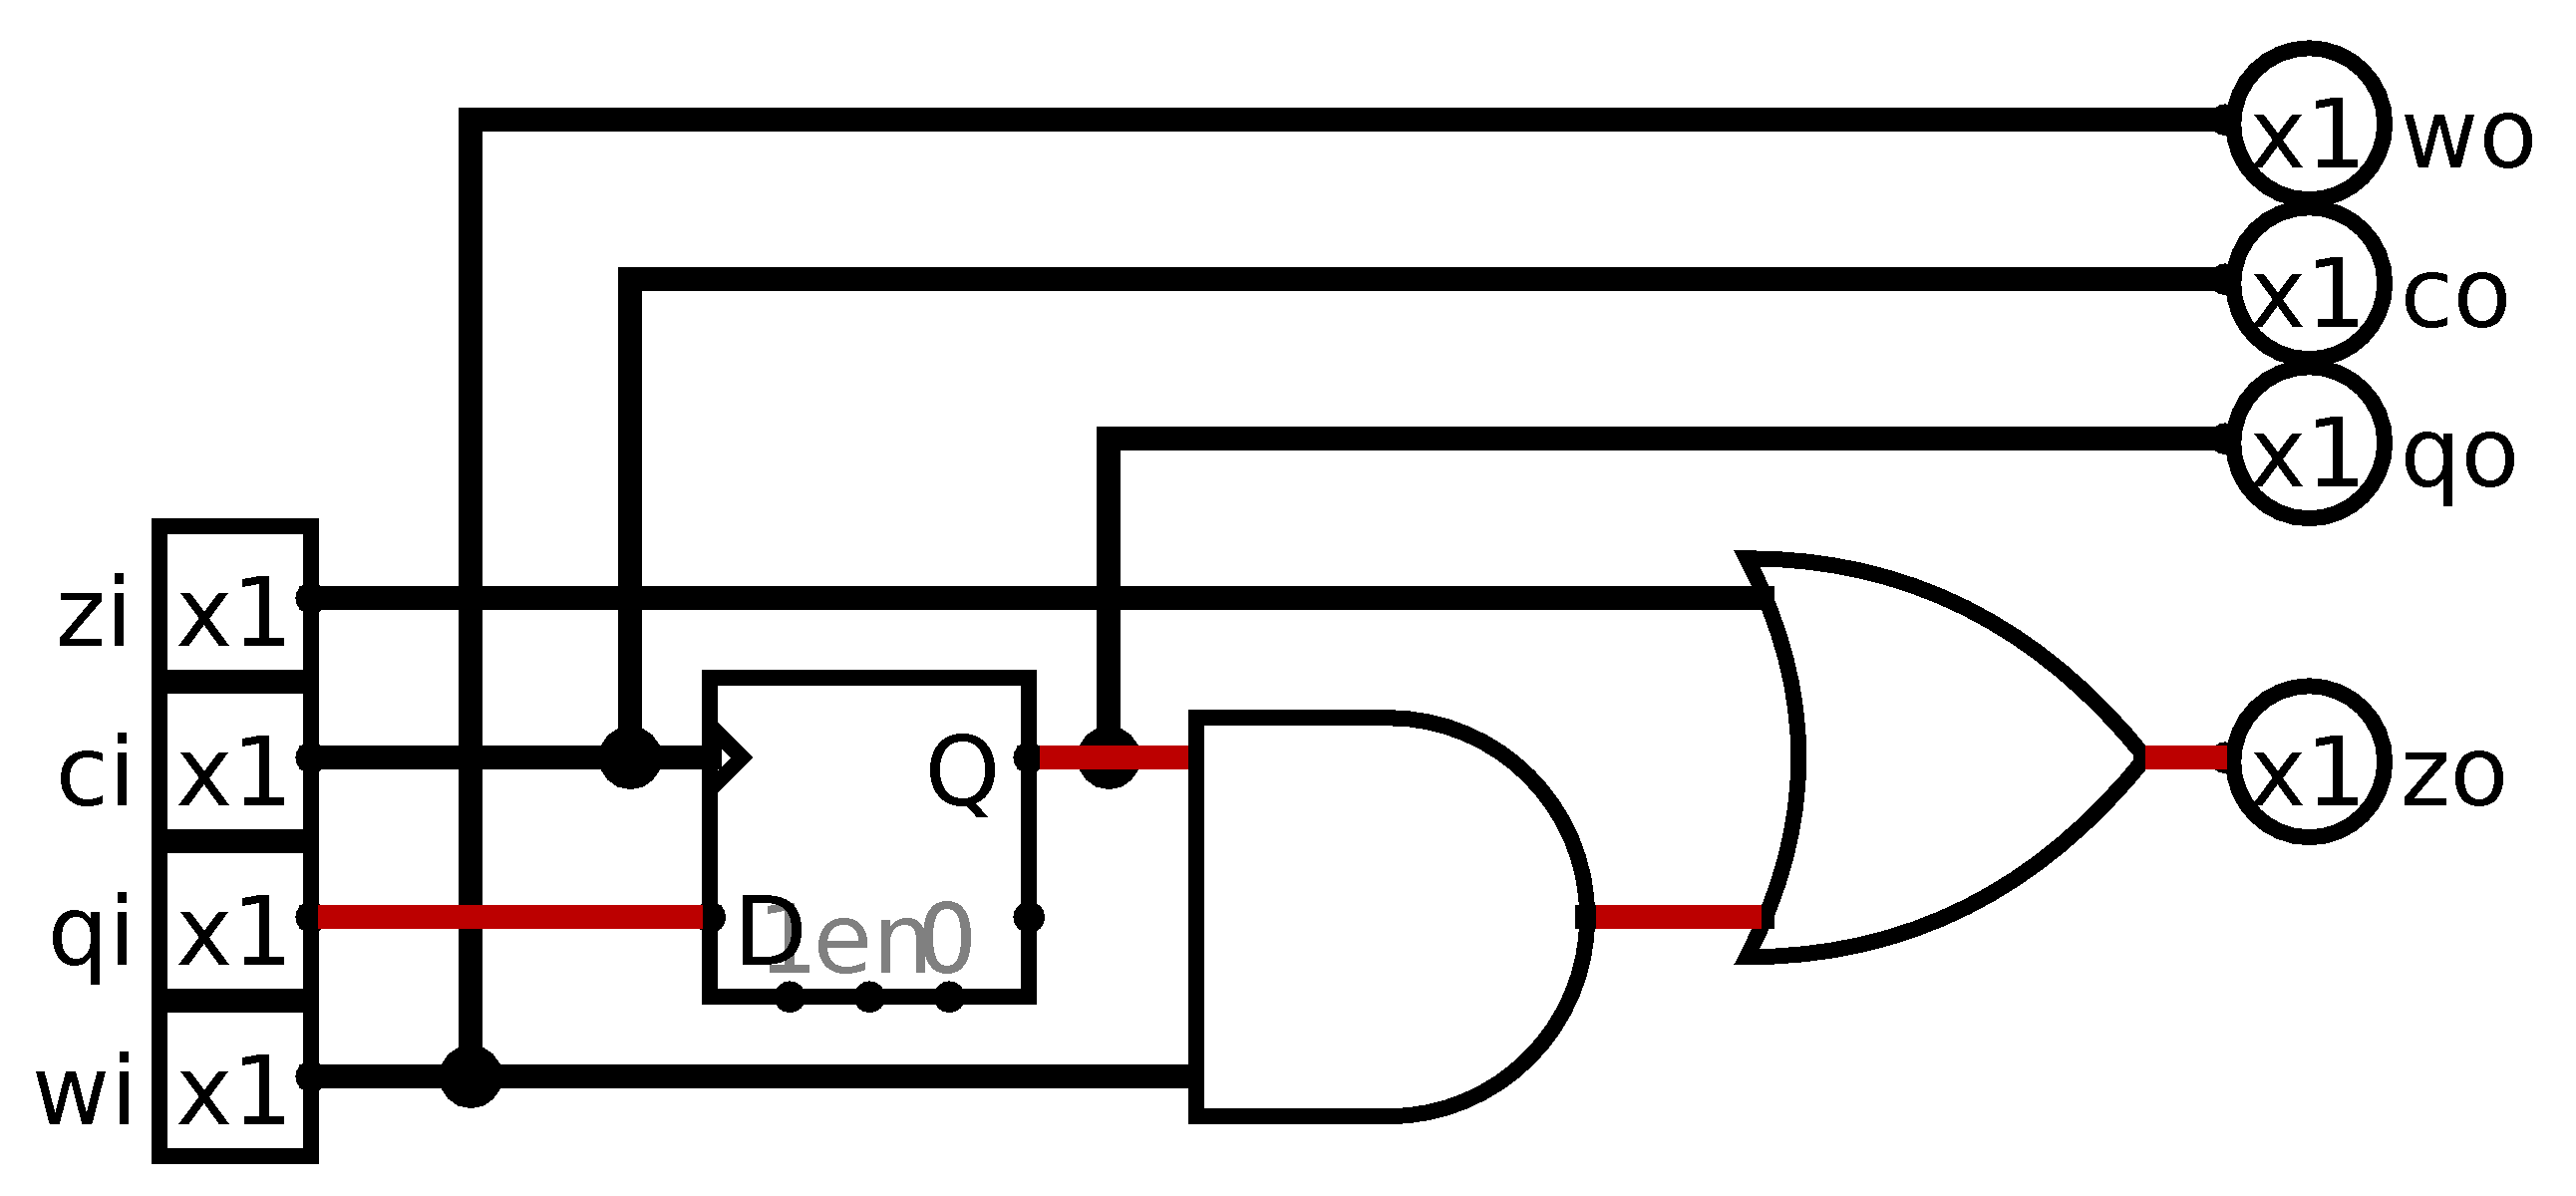
\includegraphics[width=\linewidth]{../../logisim/pin_slice_crit_path.png}
            \caption{PIN Slice Critical Path}
        \end{figure}
        \begin{figure}[H]
            \centering
            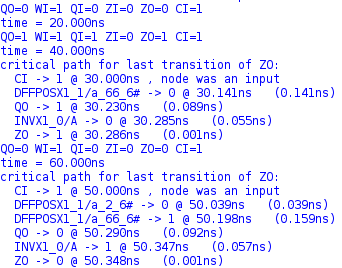
\includegraphics[]{../../irsim/pin_slice_timing.png}
            \caption{PIN Slice IRSIM Critical Path Delay}
        \end{figure}
        \begin{table}[H]
            \centering
            \begin{tabular}{crc}
                \toprule
                \textbf{State Change} & \textbf{Delay} & \\
                \midrule
                0 & 0.286n & \\
                1 & 0.348n & WORST \\
                \bottomrule
            \end{tabular}
            \caption{PIN Slice IRSIM Critical Path Delays}
        \end{table}

    \newpage
    \subsection{Shift Slice IRSIM Results}
        \lstinputlisting[caption=Python Shift Slice IRSIM CMD File Generator, language=Python]{../../irsim/shift_slice.py}
        \begin{figure}[H]
            \centering
            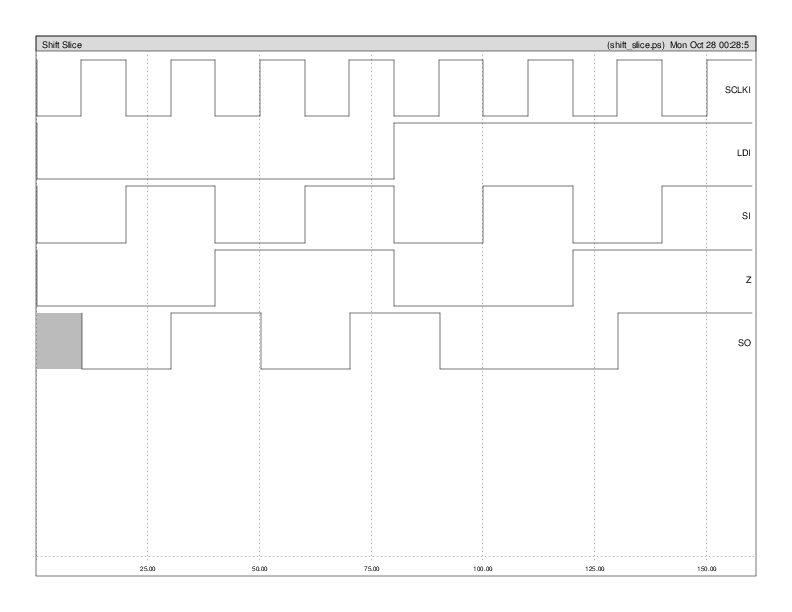
\includegraphics[width=0.75\linewidth]{../../irsim/shift_slice.png}
            \caption{Shift Slice IRSIM Functional Results}
        \end{figure}
        \begin{figure}[H]
            \centering
            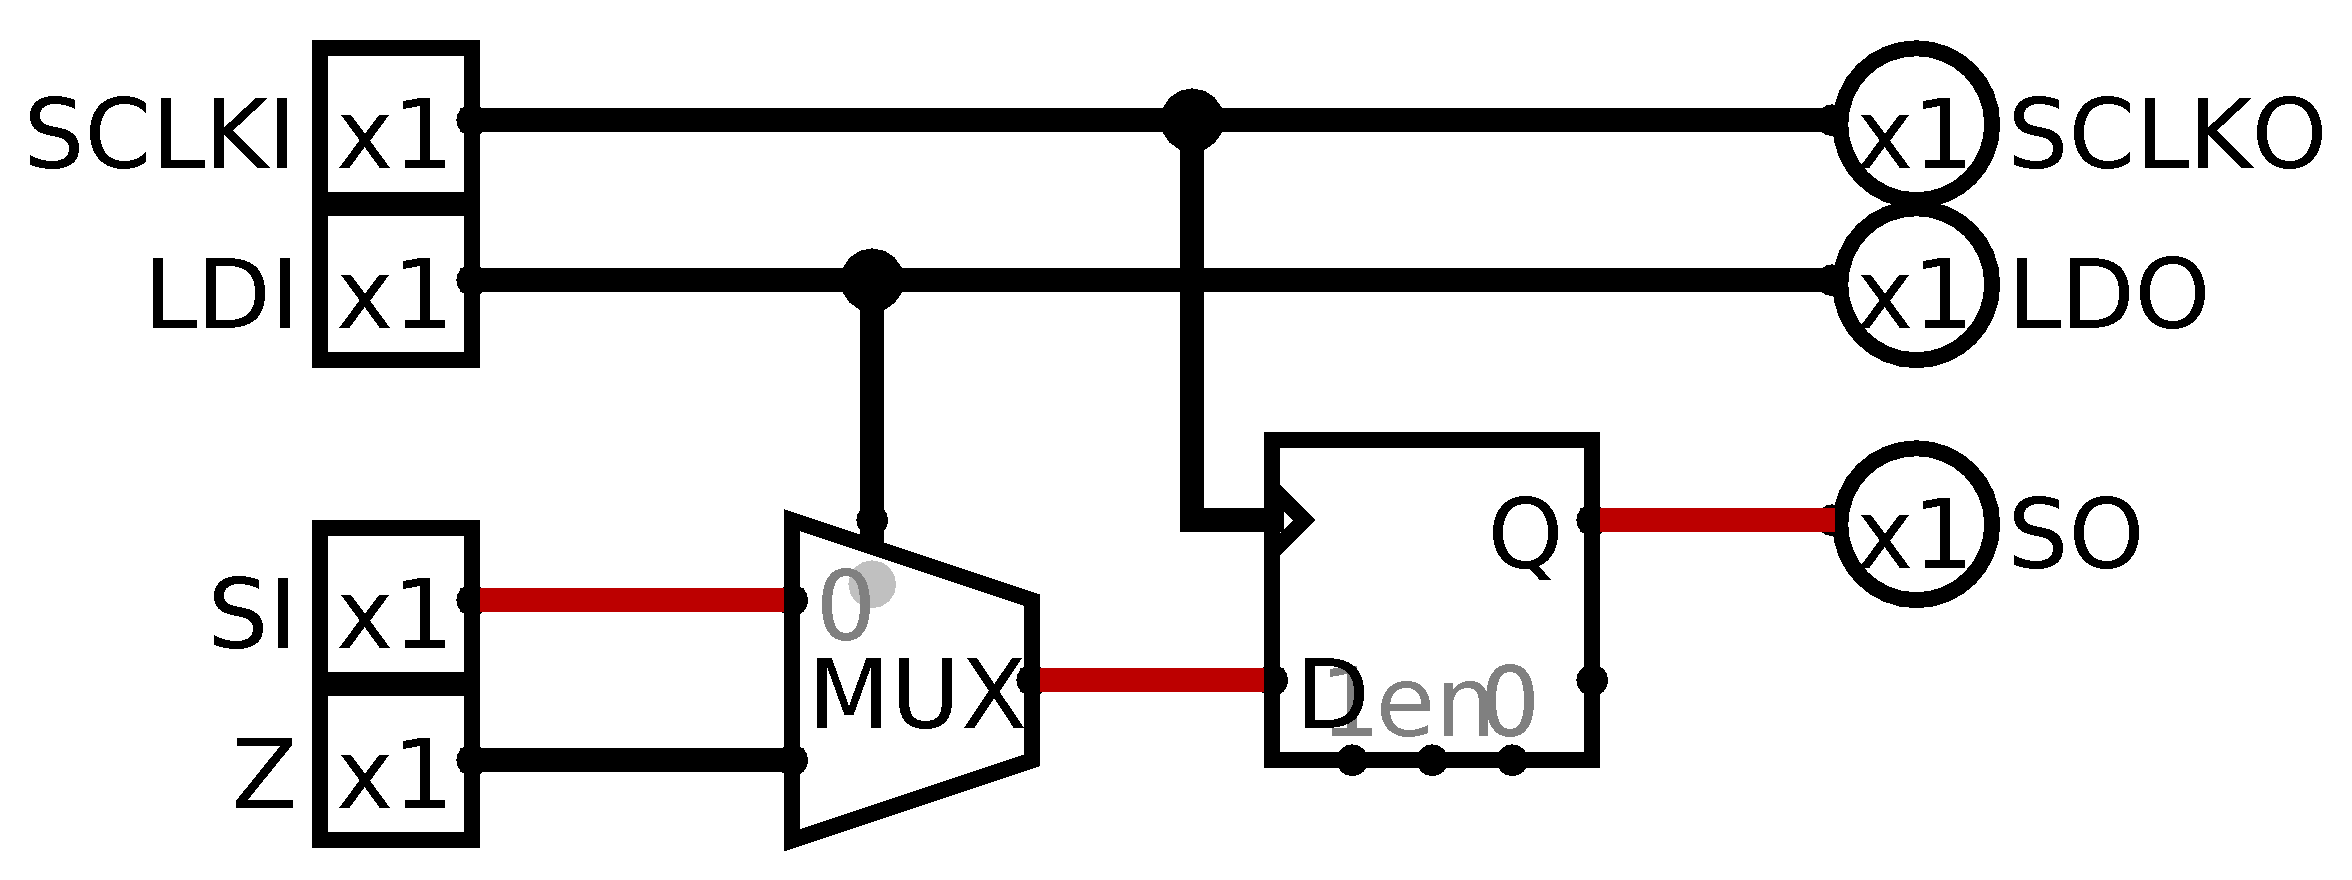
\includegraphics[width=\linewidth]{../../logisim/shift_slice_crit_path.png}
            \caption{Shift Slice Critical Path}
        \end{figure}
        \begin{figure}[H]
            \centering
            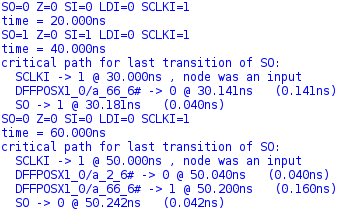
\includegraphics[]{../../irsim/shift_slice_timing.png}
            \caption{Shift Slice IRSIM Critical Path Delay}
        \end{figure}
        \begin{table}[H]
            \centering
            \begin{tabular}{crc}
                \toprule
                \textbf{State Change} & \textbf{Delay} & \\
                \midrule
                0 & 0.181n & \\
                1 & 0.242n & WORST \\
                \bottomrule
            \end{tabular}
            \caption{Shift Slice IRSIM Critical Path Delays}
        \end{table}


\newpage
\section{Spice Results}

    \subsection{PIN Slice Spice Results}
        \lstinputlisting[caption=Python PIN Slice Spice File Generator, language=Python]{../../spice/pin_slice.py}
        \begin{figure}[H]
            \centering
            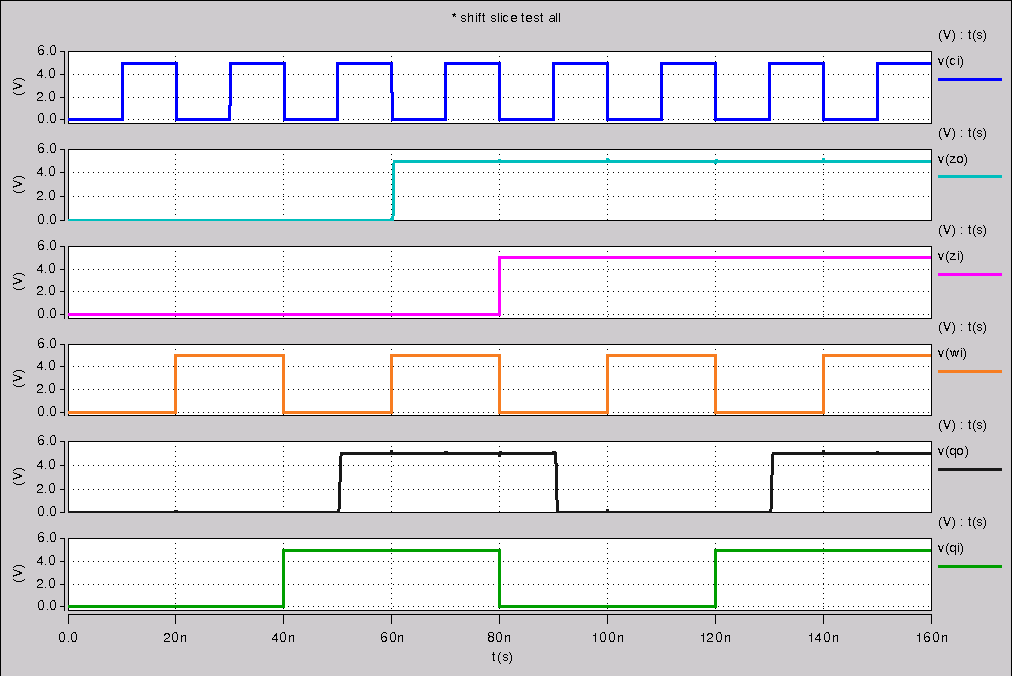
\includegraphics[width=0.75\linewidth]{../../spice/pin_slice_all.png}
            \caption{PIN Slice Spice Functional Results}
        \end{figure}
        \begin{figure}[H]
            \centering
            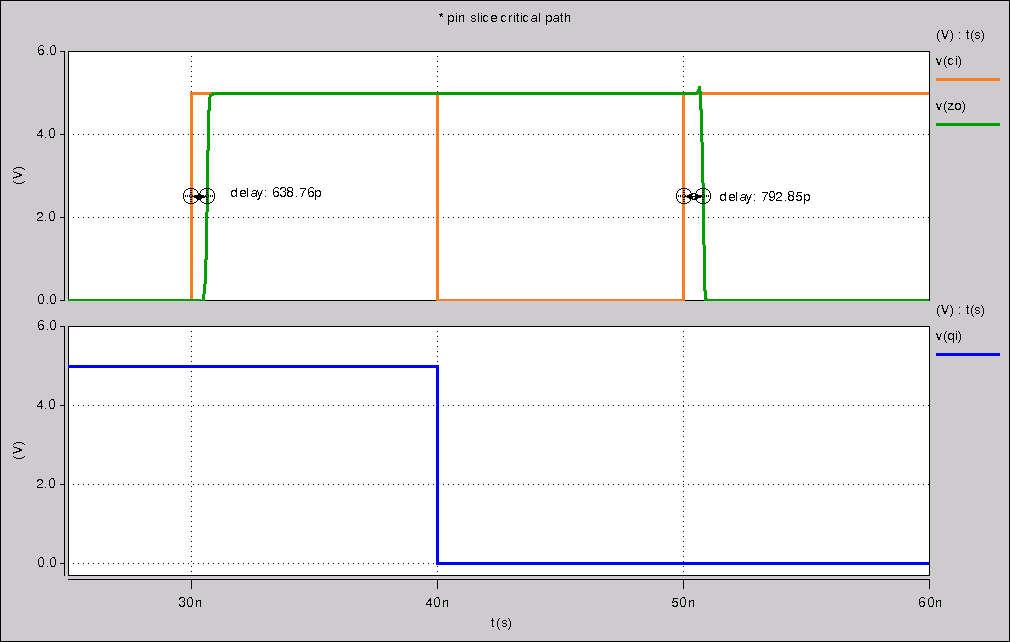
\includegraphics[width=0.75\linewidth]{../../spice/pin_slice_crit_path.png}
            \caption{PIN Slice Spice Critical Path Delay}
        \end{figure}
        \begin{table}[H]
            \centering
            \begin{tabular}{crc}
                \toprule
                \textbf{State Change} & \textbf{Delay} & \\
                \midrule
                0 & 0.638n & \\
                1 & 0.792n & WORST \\
                \bottomrule
            \end{tabular}
            \caption{PIN Slice Spice Critical Path Delays}
        \end{table}

    \newpage
    \subsection{Shift Slice Spice Results}
        \lstinputlisting[caption=Python Shift Slice Spice File Generator, language=Python]{../../spice/shift_slice.py}
        \begin{figure}[H]
            \centering
            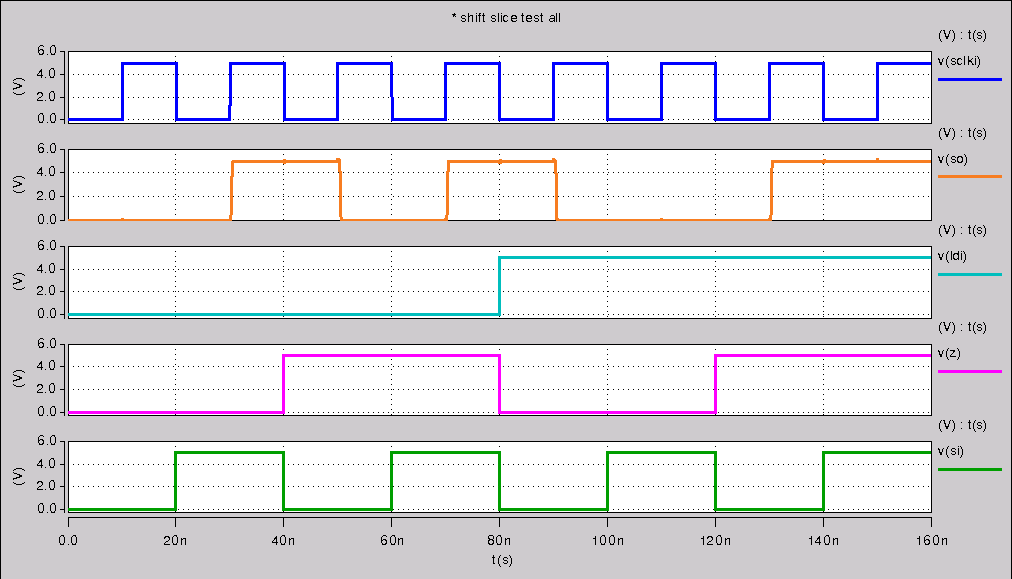
\includegraphics[width=0.75\linewidth]{../../spice/shift_slice_all.png}
            \caption{Shift Slice Spice Functional Results}
        \end{figure}
        \begin{figure}[H]
            \centering
            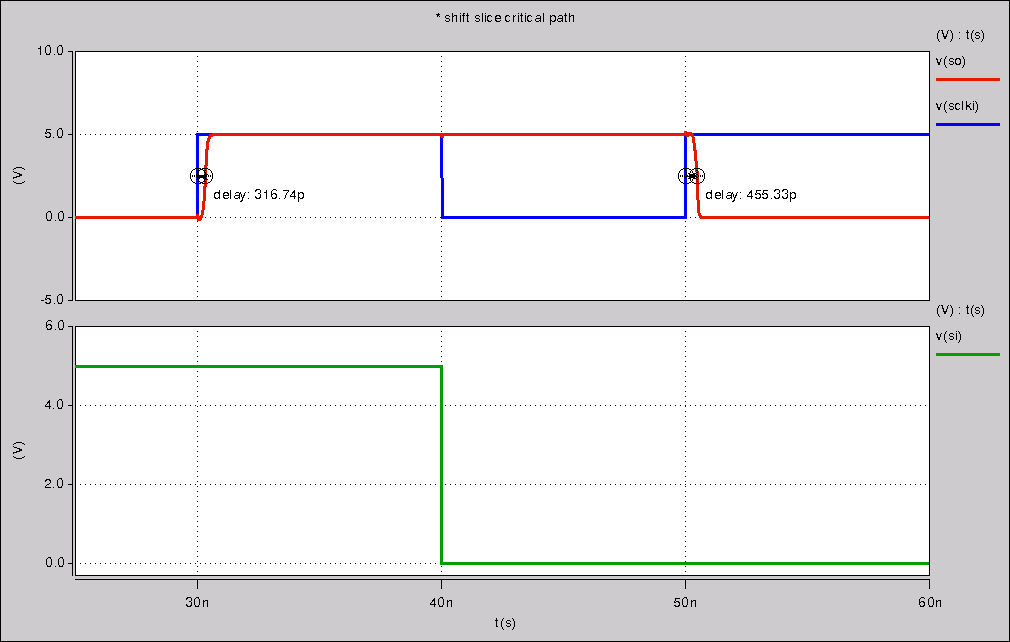
\includegraphics[width=0.75\linewidth]{../../spice/shift_slice_crit_path.png}
            \caption{Shift Slice Spice Critical Path Delay}
        \end{figure}
        \begin{table}[H]
            \centering
            \begin{tabular}{crc}
                \toprule
                \textbf{State Change} & \textbf{Delay} & \\
                \midrule
                0 & 0.316n & \\
                1 & 0.455n & WORST \\
                \bottomrule
            \end{tabular}
            \caption{Shift Slice Spice Critical Path Delays}
        \end{table}


    \newpage
    \subsection{AOI21X1 Spice Results}
        \lstinputlisting[caption=Python AOI21X1 Spice File Generator, language=Python]{../../spice/aoi21x1.py}
        \begin{figure}[H]
            \centering
            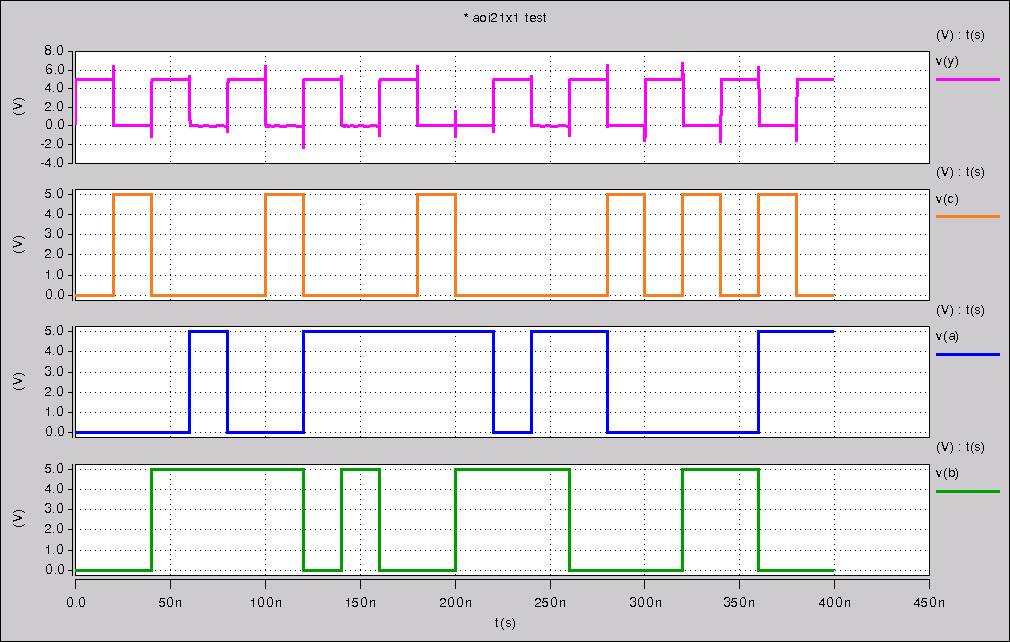
\includegraphics[width=0.75\linewidth]{../../spice/aoi21x1.png}
            \caption{AOI21X1 Spice Results}
        \end{figure}
        \begin{table}[H]
            \centering
            \begin{tabular}{crc}
                \toprule
                \textbf{State Change} & \textbf{Delay} & \\
                \midrule
                0 & 0.1075n & \\
                1 & 0.1577n & WORST \\
                2 & 0.1207n & \\
                3 & 0.1434n & \\
                4 & 0.1076n & \\
                5 & 0.1457n & \\
                6 & 0.1150n & \\
                7 & 0.0491n & \\
                8 & 0.0871n & \\
                9 & 0.0580n & \\
                \bottomrule
            \end{tabular}
            \caption{AOI21X1 Delays}
        \end{table}

    \newpage
    \subsection{DFFPOSX1 Spice Results}
        \lstinputlisting[caption=Python DFFPOSX1 Spice File Generator, language=Python]{../../spice/dffposx1.py}
        \begin{figure}[H]
            \centering
            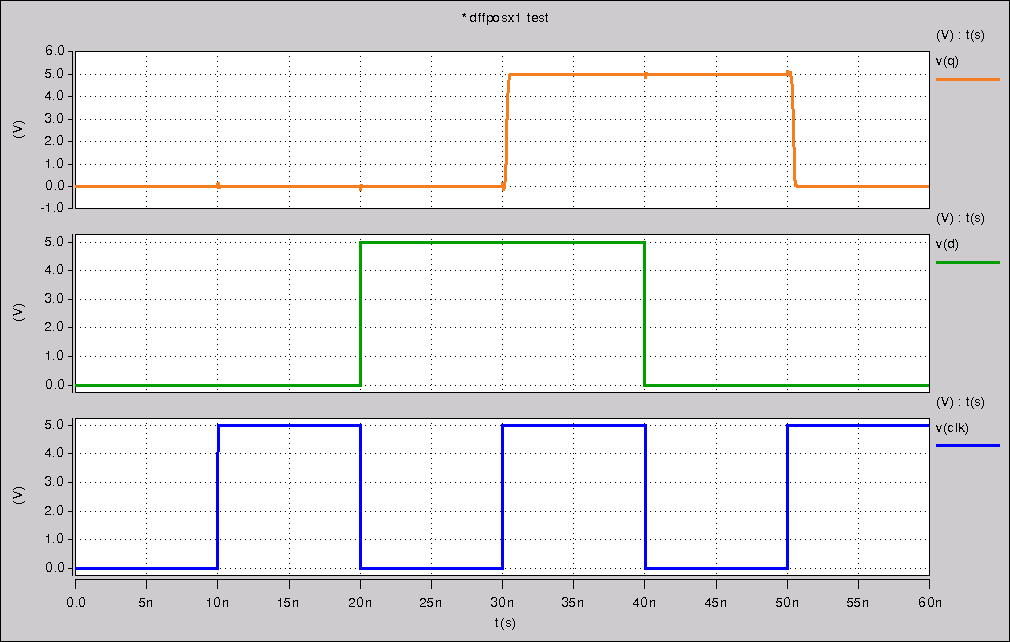
\includegraphics[width=0.75\linewidth]{../../spice/dffposx1.png}
            \caption{DFFPOSX1 Spice Results}
        \end{figure}
        \begin{table}[H]
            \centering
            \begin{tabular}{crc}
                \toprule
                \textbf{State Change} & \textbf{Delay} & \\
                \midrule
                0 & 0.3011n & \\
                1 & 0.4257n & WORST \\
                \bottomrule
            \end{tabular}
            \caption{DFFPOSX1 Delays}
        \end{table}

    \newpage
    \subsection{INVX1 Spice Results}
        \lstinputlisting[caption=Python INVX1 Spice File Generator, language=Python]{../../spice/invx1.py}
        \begin{figure}[H]
            \centering
            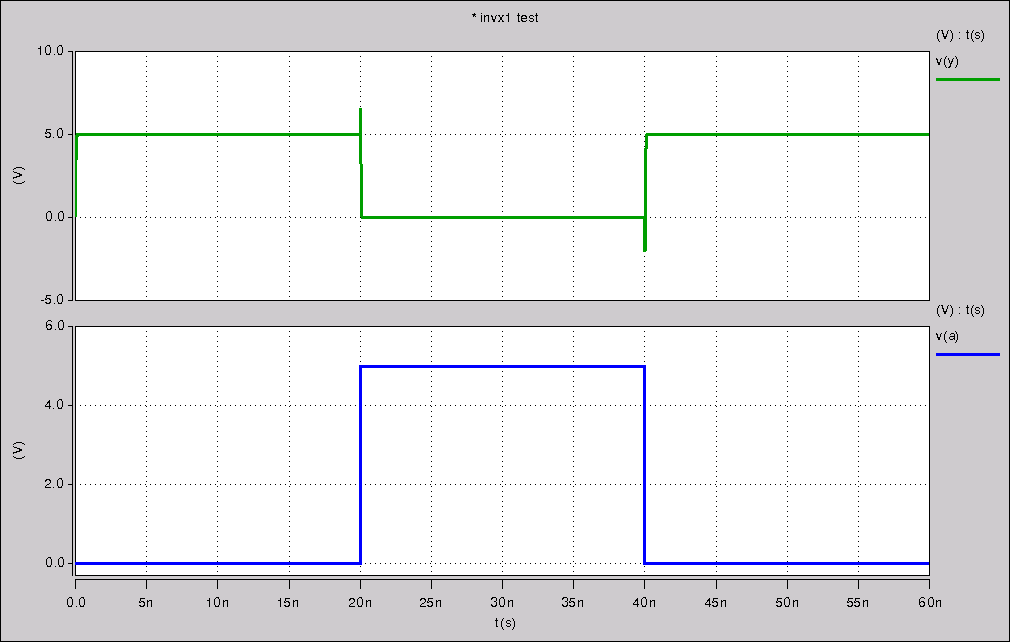
\includegraphics[width=0.75\linewidth]{../../spice/invx1.png}
            \caption{INVX1 Spice Results}
        \end{figure}
        \begin{table}[H]
            \centering
            \begin{tabular}{crc}
                \toprule
                \textbf{State Change} & \textbf{Delay} & \\
                \midrule
                0 & 0.0550n & WORST \\
                1 & 0.0407n & \\
                \bottomrule
            \end{tabular}
            \caption{INVX1 Delays}
        \end{table}

    \newpage
    \subsection{MUX2X1 Spice Results}
        \lstinputlisting[caption=Python MUX2X1 Spice File Generator, language=Python]{../../spice/mux2x1.py}
        \begin{figure}[H]
            \centering
            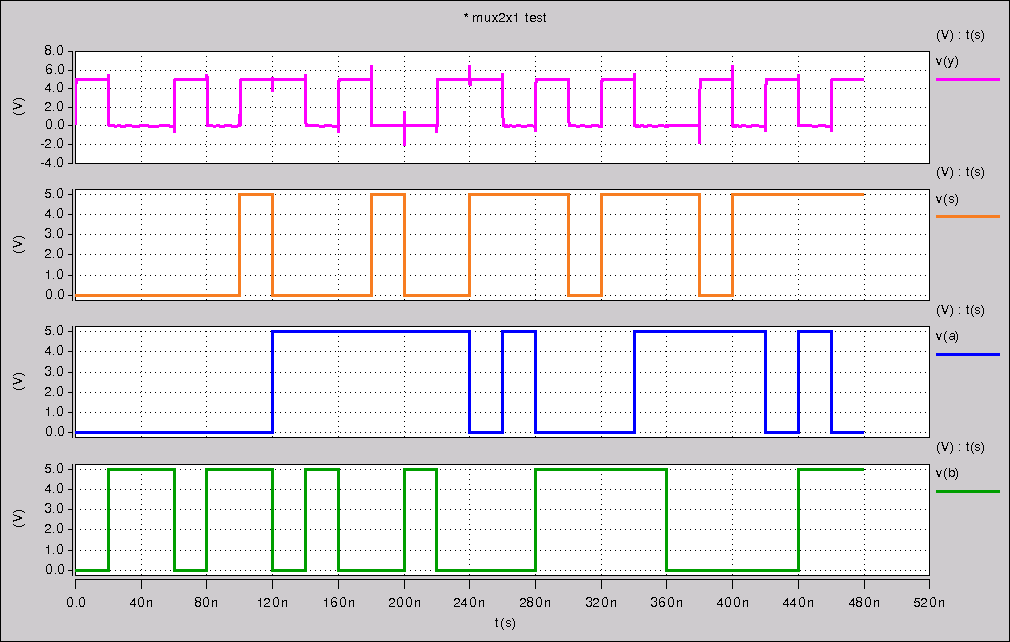
\includegraphics[width=0.75\linewidth]{../../spice/mux2x1.png}
            \caption{MUX2X1 Spice Results}
        \end{figure}
        \begin{table}[H]
            \centering
            \begin{tabular}{crc}
                \toprule
                \textbf{State Change} & \textbf{Delay} & \\
                \midrule
                0  & 0.1536n & \\
                1  & 0.1342n & \\
                2  & 0.2569n & \\
                3  & 0.1542n & \\
                4  & 0.0832n & \\
                5  & 0.1340n & \\
                6  & 0.1390n & \\
                7  & 0.2571n & WORST \\
                8  & 0.1391n & \\
                9  & 0.0788n & \\
                10 & 0.1464n & \\
                11 & 0.1467n & \\
                \bottomrule
            \end{tabular}
            \caption{MUX2X1 Delays}
        \end{table}

    \subsection{Leaf Component Delay Summary}

        \begin{table}[H]
            \centering
            \begin{tabular}{lc}
                \toprule
                \textbf{Component} & \textbf{Worst Delay} \\
                \midrule
                AOI21X1  & 0.1577n \\
                DFFPOSX1 & 0.4257n \\
                INVX1    & 0.0550n \\
                MUX2X1   & 0.2571n \\
                \bottomrule
            \end{tabular}
            \caption{Worst Case Delay Summary}
        \end{table}

\newpage
\section{VHDL Models With Timing}
    \lstinputlisting[caption=AOI21X1 VHDL Module With Delay]{../../vhdl/aoi21x1.vhd}
    \lstinputlisting[caption=DFFPOSX1 VHDL Module With Delay]{../../vhdl/dffposx1.vhd}
    \lstinputlisting[caption=INVX1 VHDL Module With Delay]{../../vhdl/invx1.vhd}
    \lstinputlisting[caption=MUX2X1 VHDL Module With Delay]{../../vhdl/mux2x1.vhd}
\section{VHDL Testbench Results With Timing}

    \subsection{VHDL Slice Testbench With Delays Waveform}

        \begin{figure}[H]
            \centering
            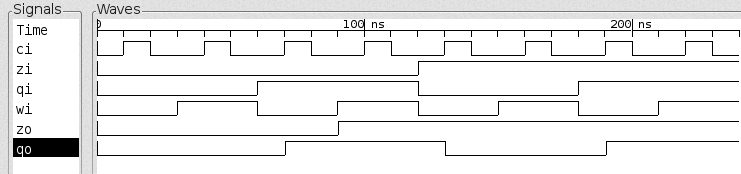
\includegraphics[width=\linewidth]{../../doc/vhdl_sim_pics/pin_slice_with_delays.png}
            \caption{VHDL PIN Slice With Delays Waveform}
        \end{figure}

        \begin{figure}[H]
            \centering
            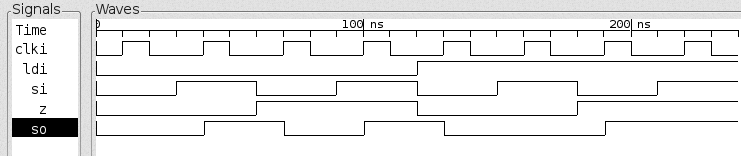
\includegraphics[width=\linewidth]{../../doc/vhdl_sim_pics/shift_slice_with_delays.png}
            \caption{VHDL Shift Slice With Delays Waveform}
        \end{figure}

    \subsection{VHDL Top Level Testbench With Delays Waveform}
        \begin{figure}[H]
            \centering
            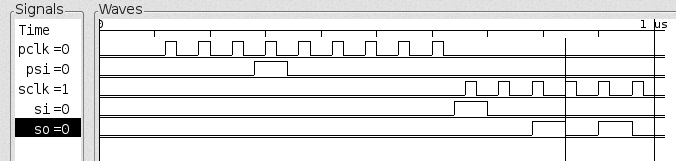
\includegraphics[width=\linewidth]{../../doc/vhdl_sim_pics/top.png}
            \caption{VHDL Top Level Functional Test Bench With Delays Waveform}
        \end{figure}

        \begin{figure}[H]
            \centering
            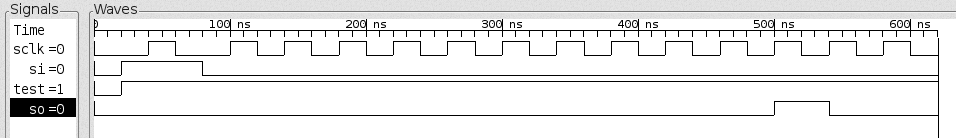
\includegraphics[width=\linewidth]{../../doc/vhdl_sim_pics/top_test.png}
            \caption{VHDL Top Level Test Mode Test Bench With Delays Waveform}
        \end{figure}

\section{Final Simulation Comparision}

        \begin{table}[H]
            \centering
            \begin{tabular}{ccc}
                \toprule
                \textbf{Simulation} & \textbf{PIN} & \textbf{Shift} \\
                \midrule
                IRSIM & 0.348n & 0.242n \\
                SPICE & 0.792n & 0.455n \\
                VHDL  & 0.638n & 0.682n \\
                \bottomrule
            \end{tabular}
            \caption{Critical Path Delay Comparison}
        \end{table}

\section{Floor Plan}
\section{Major Design Decisions}
\section{Work Division}

